% (C) Marc Lijour, 2016-2017 
% Licensed under a Creative Commons License BY-SA
% https://creativecommons.org/licenses/by-sa/2.5/ca/
% Presentation for the Small Business Digitization Initiative (SBDI) training program
% see http://www.ictc-ctic.ca/small-business-digitization-initiative/ 
% authored by Marc Lijour, December 2016
% for the session running from January 2017 to September 2017
% 
% Variables
% TODO set the variables
% ---------------------- USER-DEFINED --------------------------------
\newcommand{\SFLtitle}{Tech~Labs}
\newcommand{\SFLlongtitle}{Sharing Files and Drives in Linux}
\newcommand{\SFLsubtitle}{The short way}
\newcommand{\SFLauthor}{Marc~Lijour}
\newcommand{\SFLdate}{February~7, 2017}
\newcommand{\SFLsubject}{Tech~Labs}
% --------------------------------------------------------------------
% Template
% (C) Savoir-faire Linux, 2016 (this document and associated logos and art)
% This document is licensed under a Creative Commons License BY-SA (feel free to use the code, but all rights are reserved for logos and art)
% https://creativecommons.org/licenses/by-sa/2.5/ca/
% Savoir-faire Linux presentation template for LaTeX
% authored by Marc Lijour, December 2016
% This template comes with a first page on a blue background
% Possible improvement in future iterations
% - Test and fix as needed to work on xetex (to use Ubuntu fonts)
% === USAGE===
% Create a file for your LaTeX content (slides, etc), in which you must do the following:
% TODO 1 - set variables defined below
% TODO 2 - include this code by calling: % (C) Savoir-faire Linux, 2016 (this document and associated logos and art)
% This document is licensed under a Creative Commons License BY-SA (feel free to use the code, but all rights are reserved for logos and art)
% https://creativecommons.org/licenses/by-sa/2.5/ca/
% Savoir-faire Linux presentation template for LaTeX
% authored by Marc Lijour, December 2016
% This template comes with a first page on a blue background
% Possible improvement in future iterations
% - Test and fix as needed to work on xetex (to use Ubuntu fonts)
% === USAGE===
% Create a file for your LaTeX content (slides, etc), in which you must do the following:
% TODO 1 - set variables defined below
% TODO 2 - include this code by calling: % (C) Savoir-faire Linux, 2016 (this document and associated logos and art)
% This document is licensed under a Creative Commons License BY-SA (feel free to use the code, but all rights are reserved for logos and art)
% https://creativecommons.org/licenses/by-sa/2.5/ca/
% Savoir-faire Linux presentation template for LaTeX
% authored by Marc Lijour, December 2016
% This template comes with a first page on a blue background
% Possible improvement in future iterations
% - Test and fix as needed to work on xetex (to use Ubuntu fonts)
% === USAGE===
% Create a file for your LaTeX content (slides, etc), in which you must do the following:
% TODO 1 - set variables defined below
% TODO 2 - include this code by calling: \input{sfl-presentation-template-blue-EN}
% TODO 3 - Start the document as usual and you're in business; just use \begin{document} and don't forget to conclude with \end{document}
% TODO 4 - Use the custom method \SFLcoverpage instead of \titlepage to create your cover page
% Voilà!
%
\documentclass{beamer}
\usepackage{etoolbox}
% Variables
% ---------------------- USER-DEFINED --------------------------------
\ifdef{\SFLtitle}{}{\newcommand{\SFLtitle}{\color{red}Title TBD}}
\ifdef{\SFLlongtitle}{}{\newcommand{\SFLlongtitle}{\color{red}Long title TBD}}
\ifdef{\SFLsubtitle}{}{\newcommand{\SFLsubtitle}{\color{red}Subtitle TBD}}
\ifdef{\SFLauthor}{}{\newcommand{\SFLauthor}{\color{red}Author TBD}}
\ifdef{\SFLdate}{}{\newcommand{\SFLdate}{\color{red}Date TBD}}
\ifdef{\SFLsubject}{}{\newcommand{\SFLsubject}{\color{red}Subject TBD}}
% --------------------------------------------------------------------
\usetheme{Boadilla}
% Set color close to Savoir-faire Linux standard
\definecolor{beamer@blendedblue}{RGB}{86,176,201}
% Cover Page
\title[\SFLtitle] {\SFLlongtitle}
\subtitle{\SFLsubtitle}
\author{\SFLauthor}
\date{\SFLdate}
\subject{\SFLsubject}
\usepackage{tikz}
% -- possible approach through modif of the template (abandonned for now)
%\addtobeamertemplate{title page}{
%    \tikz[remember picture,overlay]
%        \node at ([xshift=0cm,yshift=0cm]current page.center) 
%		 {
\includegraphics[width=\paperwidth, height=\paperheight]{./images/sfl-background-blue}};
%}{}
%\setbeamercolor{title page}{fg=white}
%\setbeamercolor{titlelike}{fg=white}
%\setbeamertemplate{navigation symbols}{}
% Try Xetex to use system fonts (pdflatex makes it hard to import a font)
%\usepackage{fontspec}
%\setsansfont{Ubuntu}
%\setmonofont{Ubuntu Mono}
%
%\usepackage[absolute,overlay]{textpos}
%\setlength{\TPHorizModule}{\paperwidth}
%\setlength{\TPVertModule}{\paperheight}
% -- create a custom (command) title page -which has the benefit of not affecting the settings for the rest of the presentation
\newcommand{\SFLcoverpage}{\frame[plain]{
	\tikz[remember picture,overlay] {
        	\node(bkgd) at ([xshift=0cm,yshift=0cm]current page.center) 
			{
\includegraphics[width=\paperwidth, height=\paperheight]{../templates/images/sfl-background-blue}};
        	\node(logo) at ([xshift=0cm,yshift=2.5cm]current page.center) 
		 	{
\includegraphics[scale=.20]{../templates/images/logo-sfl-blanc-rgb-72dpi}};
	}
	\tikz[remember picture,overlay] {
        	\node(title) at ([xshift=0cm,yshift=1cm]current page.center) 
			{\Large\color{white}\textbf{{\SFLlongtitle}}};
        	\node(subtitle) at ([xshift=0cm,yshift=.2cm]current page.center) 
			{\small\color{white}\emph{\SFLsubtitle}};
        	\node(author) at ([xshift=0cm,yshift=-2cm]current page.center) 
			{\small\color{white}By~\SFLauthor};
        	\node(date) at ([xshift=0cm,yshift=-2.5cm]current page.center) 
			{\tiny\color{white}\SFLdate};
        	\node(footnote) at ([xshift=0cm,yshift=-4cm]current page.center) 
			{\TINY\color{white}\emph{The registered trademark Linux$^\circledR$ is used pursuant to a sublicense from LMI, the exclusive licensee of Linus Torvalds, owner of the mark on a world-wide basis.}};
    	}
}}
%
% This sets a Savoir-faire Linux logo at the bottom right corner of each page
\logo{
\includegraphics[scale=.1]{../templates/images/logo-sfl-250.png}}
\AtBeginSection[]
{
  \begin{frame}
    \frametitle{Table of Contents}
    \tableofcontents[currentsection]
  \end{frame}
}
%\usepackage[format=plain,justification=raggedright,singlelinecheck=false]{caption}
\usepackage[format=plain,justification=justified,singlelinecheck=false]{caption}
\usepackage[utf8]{inputenc}
\usepackage{dirtytalk}
\usepackage{wrapfig}
\usepackage{hyperref}
\usepackage{verbatim}
\usepackage{mathabx}
%\usepackage{MnSymbol}


% TODO 3 - Start the document as usual and you're in business; just use \begin{document} and don't forget to conclude with \end{document}
% TODO 4 - Use the custom method \SFLcoverpage instead of \titlepage to create your cover page
% Voilà!
%
\documentclass{beamer}
\usepackage{etoolbox}
% Variables
% ---------------------- USER-DEFINED --------------------------------
\ifdef{\SFLtitle}{}{\newcommand{\SFLtitle}{\color{red}Title TBD}}
\ifdef{\SFLlongtitle}{}{\newcommand{\SFLlongtitle}{\color{red}Long title TBD}}
\ifdef{\SFLsubtitle}{}{\newcommand{\SFLsubtitle}{\color{red}Subtitle TBD}}
\ifdef{\SFLauthor}{}{\newcommand{\SFLauthor}{\color{red}Author TBD}}
\ifdef{\SFLdate}{}{\newcommand{\SFLdate}{\color{red}Date TBD}}
\ifdef{\SFLsubject}{}{\newcommand{\SFLsubject}{\color{red}Subject TBD}}
% --------------------------------------------------------------------
\usetheme{Boadilla}
% Set color close to Savoir-faire Linux standard
\definecolor{beamer@blendedblue}{RGB}{86,176,201}
% Cover Page
\title[\SFLtitle] {\SFLlongtitle}
\subtitle{\SFLsubtitle}
\author{\SFLauthor}
\date{\SFLdate}
\subject{\SFLsubject}
\usepackage{tikz}
% -- possible approach through modif of the template (abandonned for now)
%\addtobeamertemplate{title page}{
%    \tikz[remember picture,overlay]
%        \node at ([xshift=0cm,yshift=0cm]current page.center) 
%		 {
\includegraphics[width=\paperwidth, height=\paperheight]{./images/sfl-background-blue}};
%}{}
%\setbeamercolor{title page}{fg=white}
%\setbeamercolor{titlelike}{fg=white}
%\setbeamertemplate{navigation symbols}{}
% Try Xetex to use system fonts (pdflatex makes it hard to import a font)
%\usepackage{fontspec}
%\setsansfont{Ubuntu}
%\setmonofont{Ubuntu Mono}
%
%\usepackage[absolute,overlay]{textpos}
%\setlength{\TPHorizModule}{\paperwidth}
%\setlength{\TPVertModule}{\paperheight}
% -- create a custom (command) title page -which has the benefit of not affecting the settings for the rest of the presentation
\newcommand{\SFLcoverpage}{\frame[plain]{
	\tikz[remember picture,overlay] {
        	\node(bkgd) at ([xshift=0cm,yshift=0cm]current page.center) 
			{
\includegraphics[width=\paperwidth, height=\paperheight]{../templates/images/sfl-background-blue}};
        	\node(logo) at ([xshift=0cm,yshift=2.5cm]current page.center) 
		 	{
\includegraphics[scale=.20]{../templates/images/logo-sfl-blanc-rgb-72dpi}};
	}
	\tikz[remember picture,overlay] {
        	\node(title) at ([xshift=0cm,yshift=1cm]current page.center) 
			{\Large\color{white}\textbf{{\SFLlongtitle}}};
        	\node(subtitle) at ([xshift=0cm,yshift=.2cm]current page.center) 
			{\small\color{white}\emph{\SFLsubtitle}};
        	\node(author) at ([xshift=0cm,yshift=-2cm]current page.center) 
			{\small\color{white}By~\SFLauthor};
        	\node(date) at ([xshift=0cm,yshift=-2.5cm]current page.center) 
			{\tiny\color{white}\SFLdate};
        	\node(footnote) at ([xshift=0cm,yshift=-4cm]current page.center) 
			{\TINY\color{white}\emph{The registered trademark Linux$^\circledR$ is used pursuant to a sublicense from LMI, the exclusive licensee of Linus Torvalds, owner of the mark on a world-wide basis.}};
    	}
}}
%
% This sets a Savoir-faire Linux logo at the bottom right corner of each page
\logo{
\includegraphics[scale=.1]{../templates/images/logo-sfl-250.png}}
\AtBeginSection[]
{
  \begin{frame}
    \frametitle{Table of Contents}
    \tableofcontents[currentsection]
  \end{frame}
}
%\usepackage[format=plain,justification=raggedright,singlelinecheck=false]{caption}
\usepackage[format=plain,justification=justified,singlelinecheck=false]{caption}
\usepackage[utf8]{inputenc}
\usepackage{dirtytalk}
\usepackage{wrapfig}
\usepackage{hyperref}
\usepackage{verbatim}
\usepackage{mathabx}
%\usepackage{MnSymbol}


% TODO 3 - Start the document as usual and you're in business; just use \begin{document} and don't forget to conclude with \end{document}
% TODO 4 - Use the custom method \SFLcoverpage instead of \titlepage to create your cover page
% Voilà!
%
\documentclass{beamer}
\usepackage{etoolbox}
% Variables
% ---------------------- USER-DEFINED --------------------------------
\ifdef{\SFLtitle}{}{\newcommand{\SFLtitle}{\color{red}Title TBD}}
\ifdef{\SFLlongtitle}{}{\newcommand{\SFLlongtitle}{\color{red}Long title TBD}}
\ifdef{\SFLsubtitle}{}{\newcommand{\SFLsubtitle}{\color{red}Subtitle TBD}}
\ifdef{\SFLauthor}{}{\newcommand{\SFLauthor}{\color{red}Author TBD}}
\ifdef{\SFLdate}{}{\newcommand{\SFLdate}{\color{red}Date TBD}}
\ifdef{\SFLsubject}{}{\newcommand{\SFLsubject}{\color{red}Subject TBD}}
% --------------------------------------------------------------------
\usetheme{Boadilla}
% Set color close to Savoir-faire Linux standard
\definecolor{beamer@blendedblue}{RGB}{86,176,201}
% Cover Page
\title[\SFLtitle] {\SFLlongtitle}
\subtitle{\SFLsubtitle}
\author{\SFLauthor}
\date{\SFLdate}
\subject{\SFLsubject}
\usepackage{tikz}
% -- possible approach through modif of the template (abandonned for now)
%\addtobeamertemplate{title page}{
%    \tikz[remember picture,overlay]
%        \node at ([xshift=0cm,yshift=0cm]current page.center) 
%		 {
\includegraphics[width=\paperwidth, height=\paperheight]{./images/sfl-background-blue}};
%}{}
%\setbeamercolor{title page}{fg=white}
%\setbeamercolor{titlelike}{fg=white}
%\setbeamertemplate{navigation symbols}{}
% Try Xetex to use system fonts (pdflatex makes it hard to import a font)
%\usepackage{fontspec}
%\setsansfont{Ubuntu}
%\setmonofont{Ubuntu Mono}
%
%\usepackage[absolute,overlay]{textpos}
%\setlength{\TPHorizModule}{\paperwidth}
%\setlength{\TPVertModule}{\paperheight}
% -- create a custom (command) title page -which has the benefit of not affecting the settings for the rest of the presentation
\newcommand{\SFLcoverpage}{\frame[plain]{
	\tikz[remember picture,overlay] {
        	\node(bkgd) at ([xshift=0cm,yshift=0cm]current page.center) 
			{
\includegraphics[width=\paperwidth, height=\paperheight]{../templates/images/sfl-background-blue}};
        	\node(logo) at ([xshift=0cm,yshift=2.5cm]current page.center) 
		 	{
\includegraphics[scale=.20]{../templates/images/logo-sfl-blanc-rgb-72dpi}};
        	\node(CC-BY-SA) at ([xshift=5cm,yshift=-3.5cm]current page.center) 
			{\href{https://creativecommons.org/licenses/by-sa/2.5/ca/}{
\includegraphics[scale=.4]{../templates/images/CC-BY-SA-403x141}}};
	}
	\tikz[remember picture,overlay] {
        	\node(title) at ([xshift=0cm,yshift=1cm]current page.center) 
			{\Large\color{white}\textbf{{\SFLlongtitle}}};
        	\node(subtitle) at ([xshift=0cm,yshift=.2cm]current page.center) 
			{\small\color{white}\emph{\SFLsubtitle}};
        	\node(author) at ([xshift=0cm,yshift=-2cm]current page.center) 
			{\small\color{white}By~\SFLauthor};
        	\node(date) at ([xshift=0cm,yshift=-2.5cm]current page.center) 
			{\tiny\color{white}\SFLdate};
        	\node(footnote) at ([xshift=0cm,yshift=-4cm]current page.center) 
			{\TINY\color{white}\emph{The registered trademark Linux$^\circledR$ is used pursuant to a sublicense from LMI, the exclusive licensee of Linus Torvalds, owner of the mark on a world-wide basis.}};
    	}
}}
%
% This sets a Savoir-faire Linux logo at the bottom right corner of each page
\logo{
	
\includegraphics[scale=.1]{../templates/images/logo-sfl-250.png}
}
\AtBeginSection[]
{
  \begin{frame}
    \frametitle{Table of Contents}
    \tableofcontents[currentsection]
  \end{frame}
}
%\usepackage[format=plain,justification=raggedright,singlelinecheck=false]{caption}
\usepackage[format=plain,justification=justified,singlelinecheck=false]{caption}
\usepackage[utf8]{inputenc}
\usepackage{dirtytalk}
\usepackage{wrapfig}
\usepackage{hyperref}
\usepackage{verbatim}
\usepackage{mathabx}
%\usepackage{MnSymbol}


% Extra packages
\usepackage{amssymb}
\usepackage{amsmath}
\usepackage[american]{babel}
\usepackage{csquotes}
\usepackage[backend=biber,style=apa]{biblatex}
\DeclareLanguageMapping{american}{american-apa}
% Use one bib file per section
\addbibresource{references-shared-drives.bib}
\definecolor{links}{HTML}{2A1B81}
\hypersetup{colorlinks,linkcolor=,urlcolor=links}
% Start of the document
\begin{document}
% Cover page
% Do not use this: \frame{\titlepage}
% use this instead:
\SFLcoverpage

% ======================================================================================================
%                                  SHARED DRIVES 
% ======================================================================================================
\section{Sharing a Drive}
% --------------------- Sources of Innovation --------------------------
\frame{
	\frametitle{Purpose}
	\begin{itemize}
		\item Share some files with people who use Linux, Windows, or other
		\item Share files between machines
		\item Make files accessible throughout your home or office (but not outside those walls)
	\end{itemize}
}

\frame{
	\frametitle{Open the Sharing Options (right-click)}
        \begin{figure}
		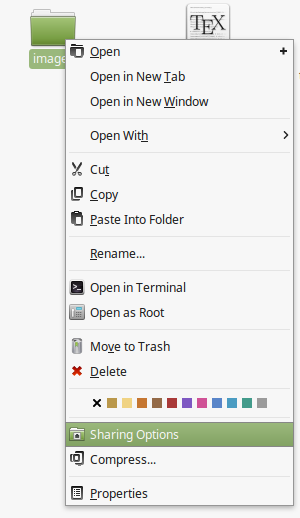
\includegraphics[height=7cm]{../pics/drive-right-click}
	\end{figure}
}

\frame{
	\frametitle{Folder Properties}
        \begin{figure}
		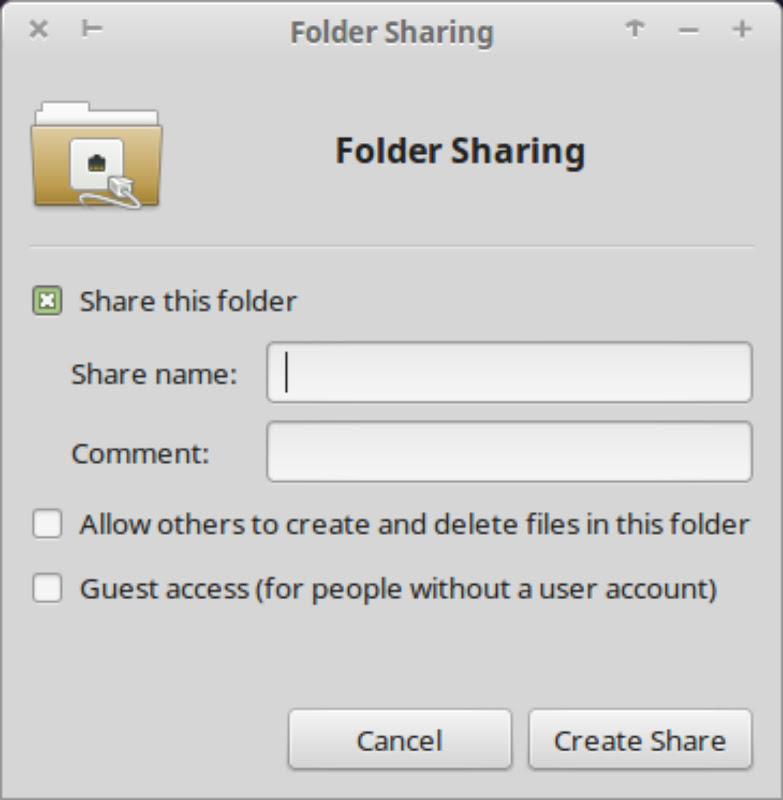
\includegraphics[height=7cm]{../pics/drive-4-share}
		\caption{Pic and guidance from \cite{magicmint}}
	\end{figure}

}

\frame{
	\frametitle{Fix a few details}
	\framesubtitle{Install Samba, the SMB file server, \& create the expected folder with the right permissions}
%	\begin{exampleblock}{Type this as root}
		\texttt{\$ sudo su - \# to become root \\
			\# apt-get install samba \\
			\# /etc/init.d/samba restart \\
			\# mkdir /var/lib/samba/usershares/ \\
			\# chmod 1775 /var/lib/samba/usershares/ \\
			\# chown root:sambashare /var/lib/samba/usershares/ \\
			\# service samba restart \# or try /etc/init.d/samba restart \\
			\# exit
		}
%	\end{exampleblock}
}

\frame{
	\frametitle{Update the firewall configuration (if you have one set up)}
		\texttt{\$ sudo ufw allow samba}
}

\frame{
	\frametitle{Another potential fix}
	\framesubtitle{In case your computer has a long name ($>$ 15 characters)}
	Samba prefers short names (less than 15 characters). Add the following line in /etc/samba/smb.conf, just after the line with ``server string\ldots'':\\
	\hspace{5em}\texttt{netbios name = Whatever}\\
	(Change \texttt{Whatever} by whatever you want your computer name to be.)\\
	\vspace{3em}
%	\begin{exampleblock}{Type this as root}
		\texttt{\$ sudo su - \# to become root \\
			\# gedit /etc/samba/smb.conf \\
			\# exit \\
		}
%	\end{exampleblock}
}

\frame{
	\frametitle{Browse the Network (same computer or another)}
	\framesubtitle{Click on ``Windows Network'' and keep clicking under you see your folders}
        \begin{figure}
		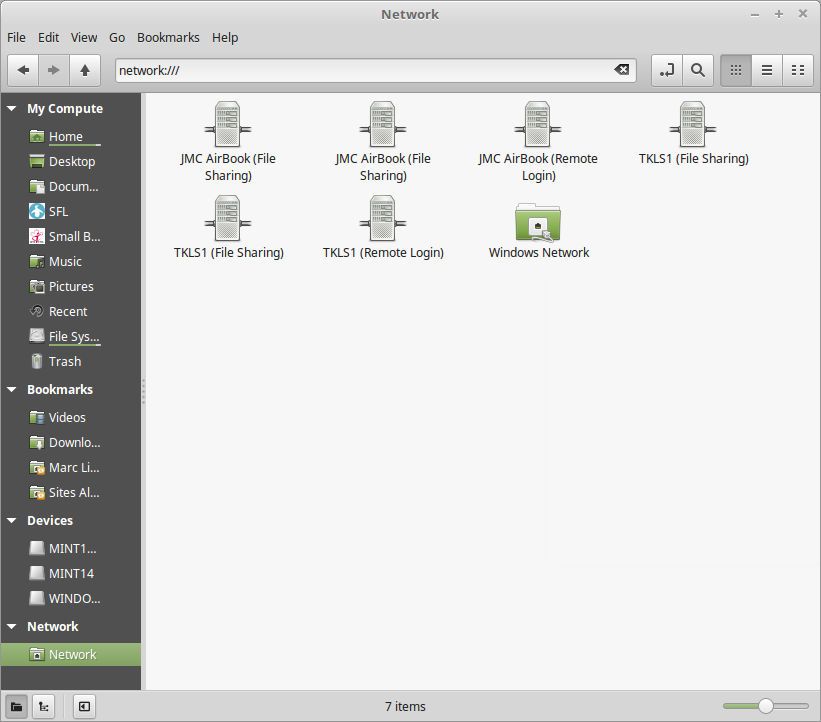
\includegraphics[height=7cm]{../pics/nemo-network}
	\end{figure}
}

\section{More things you can do}
% --------------------- Extra / Other things ------------------
\frame{
	\frametitle{Set a Work Group}
	\framesubtitle{Let's create our own ``SBDI'' group}
	You need to edit the config file \texttt{/etc/samba/smb.conf} \\
	\vspace{2em}
		\texttt{\$ sudo su - \# to become root \\
			\# gedit /etc/samba/smb.conf \\
			\# exit \\
		}
	\vspace{2em}
	After ``workgroup = '', change \texttt{WORKGROUP} for \texttt{SBDI}. Save the file and restart Samba.\\
	\vspace{2em}
	\texttt{\$ sudo /etc/init.d/samba restart}  \\
}

\frame{
	\frametitle{Debugging}
	\framesubtitle{Get information on what's going on}
	\texttt{\$ testparm -s \\
		\$ net usershare info --long \\
	}
	\vspace{3em}
	For more information see \cite{ubunturefshares}
}

\section{References}
% --------------------- References --------------------------
\frame{
	\frametitle{References}
	\printbibliography	
}


\end{document}

